% Appendix
\section{Schematics and Electrical Drawings}
\label{app:schematics}

This section includes the electrical schematics and wiring diagrams for the Factory Alcohol Detection System.

\subsection{Circuit Diagram}
The circuit diagram for the system is shown in Figure~\ref{fig:circuit_diagram}. It includes the connections for the following components:
\begin{itemize}
    \item Arduino Uno R3 microcontroller.
    \item MQ-3 alcohol sensor.
    \item FPM10A fingerprint reader.
    \item 24V DC electric door locks.
    \item 85 dB buzzer and LED indicators.
    \item SD card module for data logging.
\end{itemize}

\begin{figure}[H]
    \centering
    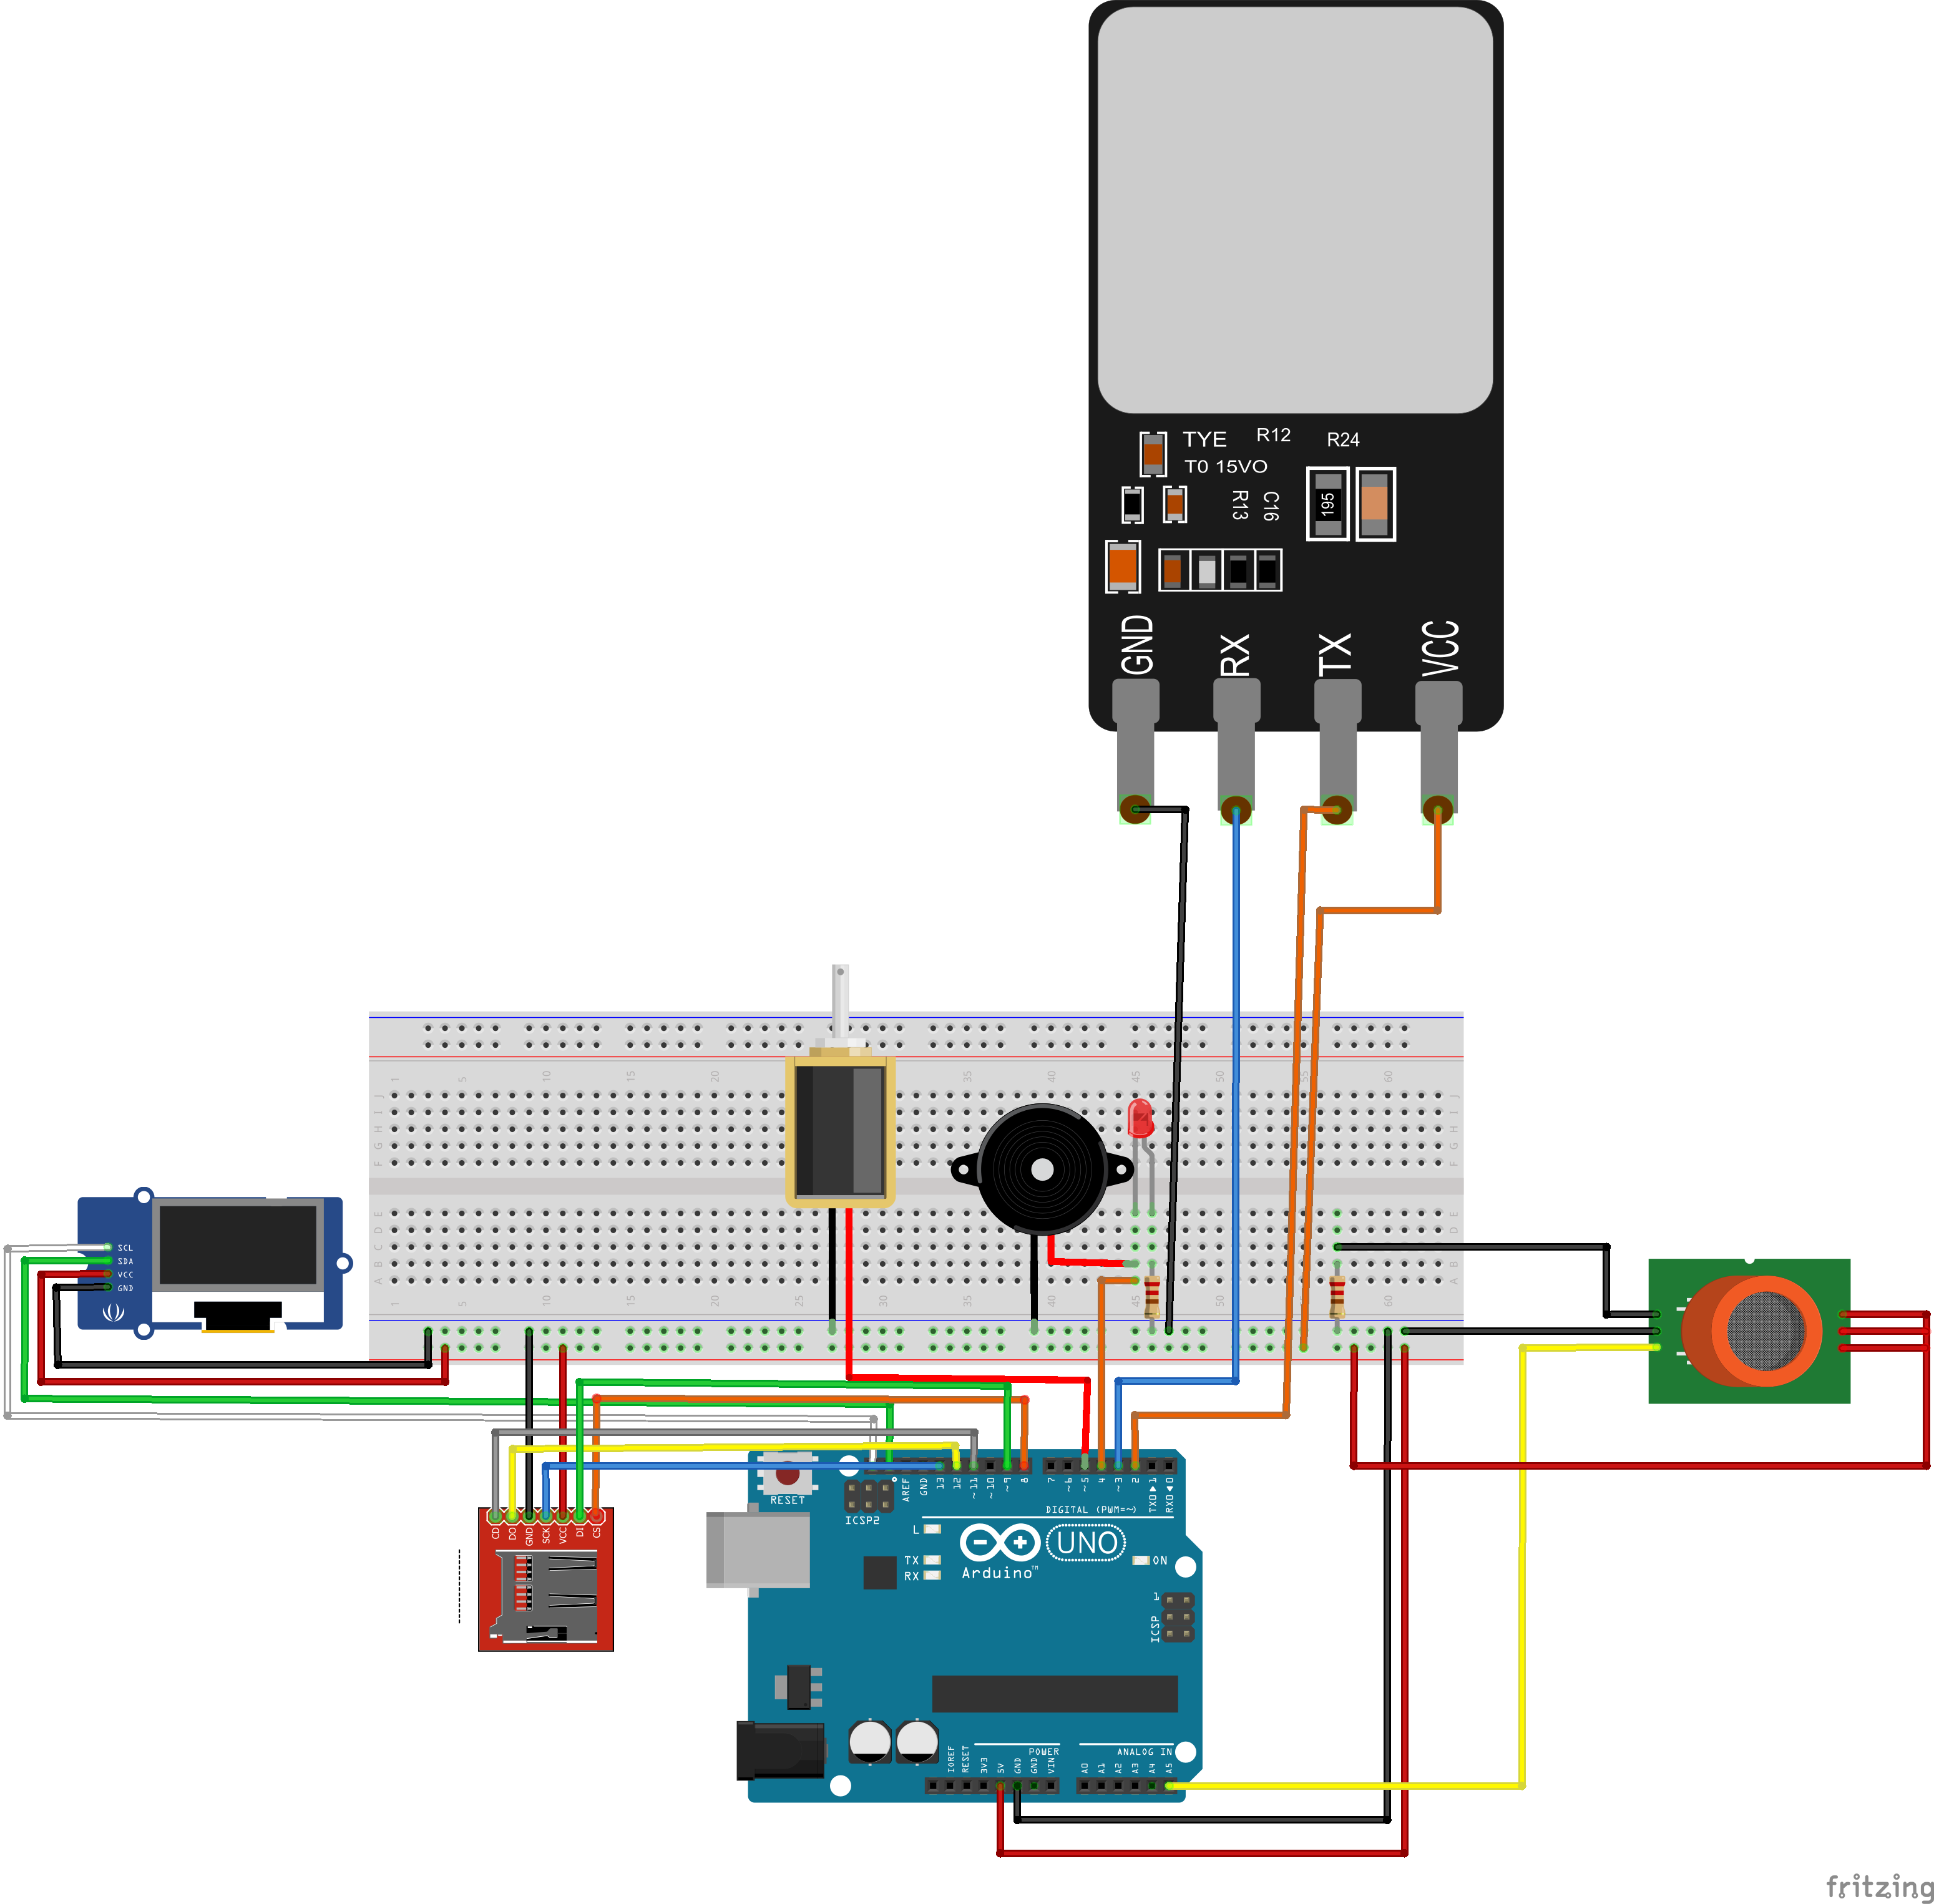
\includegraphics[width=0.8\textwidth]{images/circuit_diagram.png}
    \caption{Circuit Diagram of the Alcohol Detection System}
    \label{fig:circuit_diagram}
\end{figure}
\begin{figure}[H]
    \centering
    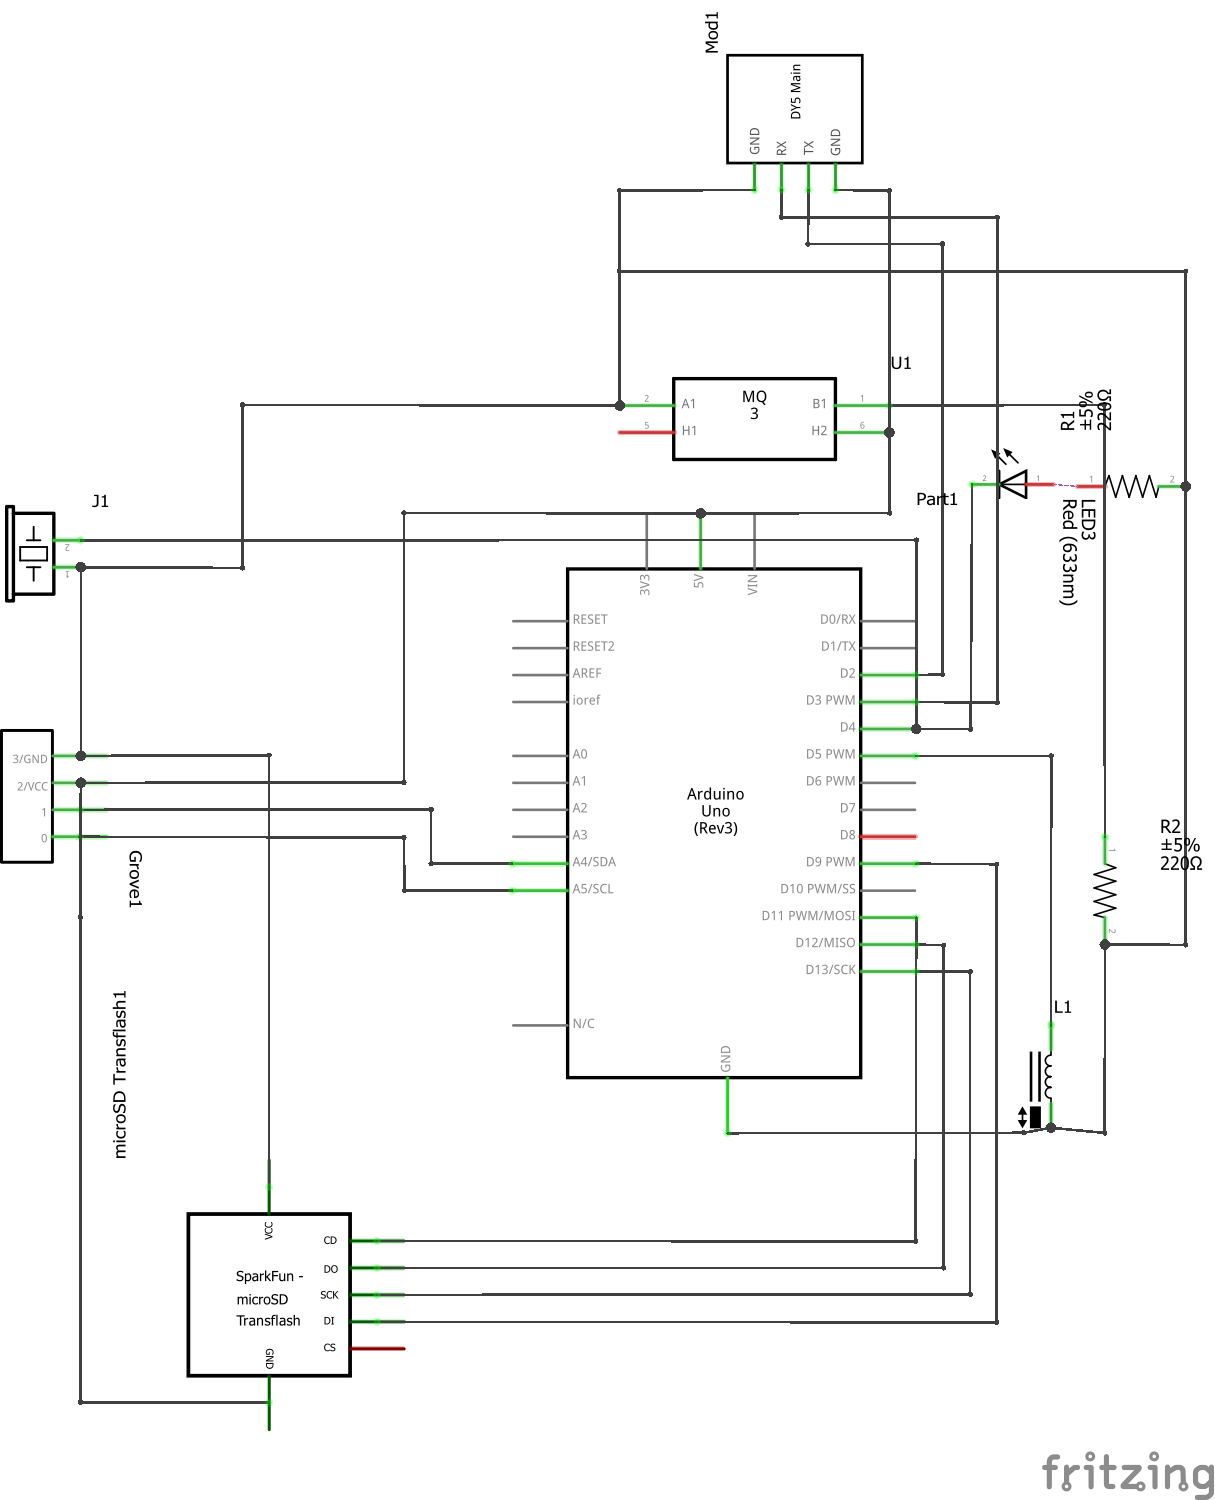
\includegraphics[width=0.8\textwidth]{images/schematic.png}
    \caption{Schematic Diagram of the Alcohol Detection System}
    \label{fig:schematic_diagram}
\end{figure}

\subsection{Power Supply Design}
The power supply circuit provides 24V DC to the system. It includes:
\begin{itemize}
    \item A voltage regulator to ensure stable power delivery.
    \item Overcurrent and overvoltage protection circuits.
\end{itemize}

\section{Mechanical Drawings}
\label{app:mechanical_drawings}

This section includes the image for the mantrap structure and breathalyzer.

\begin{figure}[H]
    \centering
    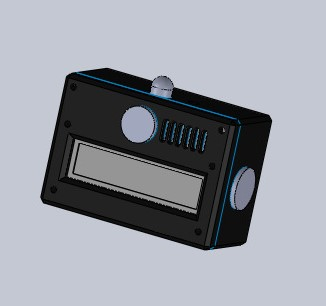
\includegraphics[width=0.5\textwidth]{images/assembly.JPG}
    \caption{Diagram of the Alcohol Detection System Enclosure}
    \label{fig:3d_diagram}
\end{figure}

\subsection{Mantrap Structure}
The mantrap structure is designed to ensure controlled entry and exit of employees. Key features include:
\begin{itemize}
    \item Secure enclosure with entry and exit gates.
    \item Testing chamber for breath sample collection.
\end{itemize}

\begin{figure}[H]
    \centering
    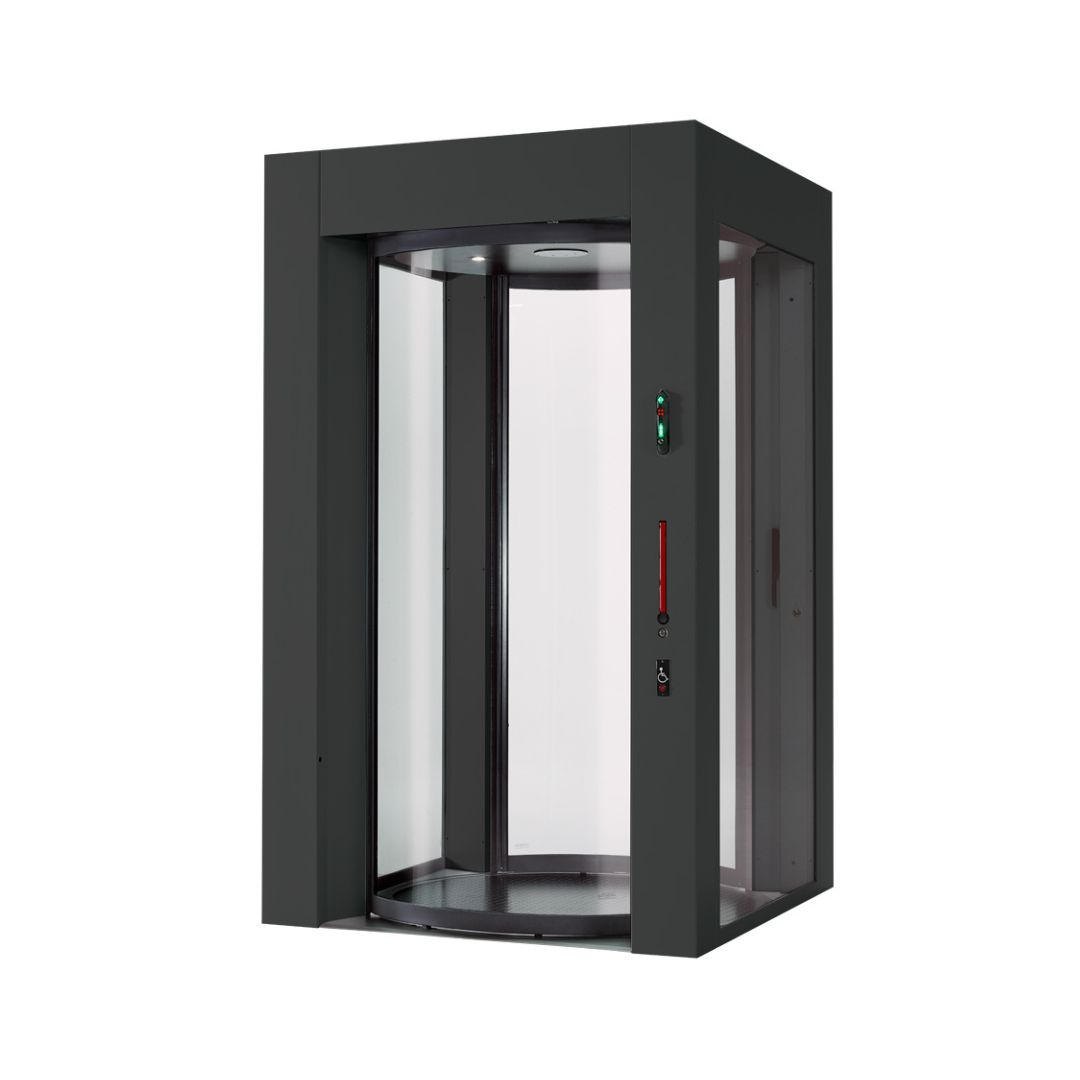
\includegraphics[width=0.5\textwidth]{images/mantrap_drawing.png}
    \caption{Picture of the Mantrap Structure}
    \label{fig:mantrap_drawing}
\end{figure}

%\subsection{Gate Mechanism}
%The gate mechanism is powered by 24V DC electric door %locks. It includes:
%\begin{itemize}
%    \item Electrically controlled doors with a response time of $\leq 2$ seconds.
%    \item Safety sensors to prevent accidental closure.
%\end{itemize}

\section{Source Code}
\label{app:source_code}

This section provides the source code for the Factory Alcohol Detection System. The code is written for the Arduino Uno R3 microcontroller.

\subsection{Main Program}
The main program handles data acquisition, decision-making, and logging. Key functionalities include:
\begin{itemize}
    \item Reading data from the MQ-3 alcohol sensor.
    \item Verifying employee identity using the FPM10A fingerprint reader.
    \item Controlling the gate mechanism and alarm system.
    \item Logging incidents to the SD card.
\end{itemize}

\begin{lstlisting}[language=C++, caption={Main Program for Alcohol Detection System}]
#include <SoftwareSerial.h>
#include <SD.h>
#include <FPM.h>

// Pin definitions
const int alcoholSensorPin = A0;
const int gateLockPin = 9;
const int buzzerPin = 10;
const int ledPin = 11;

// Variables
float alcoholLevel;
bool accessGranted = false;

void setup() {
    // Initialize components
    pinMode(alcoholSensorPin, INPUT);
    pinMode(gateLockPin, OUTPUT);
    pinMode(buzzerPin, OUTPUT);
    pinMode(ledPin, OUTPUT);
    Serial.begin(9600);

    // Initialize SD card
    if (!SD.begin(4)) {
        Serial.println("SD card initialization failed!");
        return;
    }
}

void loop() {
    // Read alcohol level
    alcoholLevel = analogRead(alcoholSensorPin) * (5.0 / 1023.0);

    // Check alcohol level
    if (alcoholLevel <= 0.02) {
        accessGranted = true;
        digitalWrite(gateLockPin, HIGH); // Open gate
        digitalWrite(buzzerPin, LOW);    // Turn off alarm
        digitalWrite(ledPin, LOW);       // Turn off LED
    } else {
        accessGranted = false;
        digitalWrite(gateLockPin, LOW);  // Close gate
        digitalWrite(buzzerPin, HIGH);   // Turn on alarm
        digitalWrite(ledPin, HIGH);      // Turn on LED
    }

    // Log incident
    logIncident(alcoholLevel, accessGranted);
    delay(1000);
}

void logIncident(float alcoholLevel, bool accessGranted) {
    File dataFile = SD.open("log.txt", FILE_WRITE);
    if (dataFile) {
        dataFile.print("Alcohol Level: ");
        dataFile.print(alcoholLevel);
        dataFile.print(", Access Granted: ");
        dataFile.println(accessGranted ? "Yes" : "No");
        dataFile.close();
    } else {
        Serial.println("Error opening log file!");
    }
}
\end{lstlisting}

\subsection{Libraries Used}
The following libraries are used in the program:
\begin{itemize}
    \item \texttt{SoftwareSerial.h}: For serial communication with the fingerprint reader.
    \item \texttt{SD.h}: For interfacing with the SD card module.
    \item \texttt{FPM.h}: For interfacing with the FPM10A fingerprint reader.
\end{itemize}